%!TeX root=../pridetop.tex
\chapter[Chapter \thechapter]{}
\begin{figure}[t!]
\centering
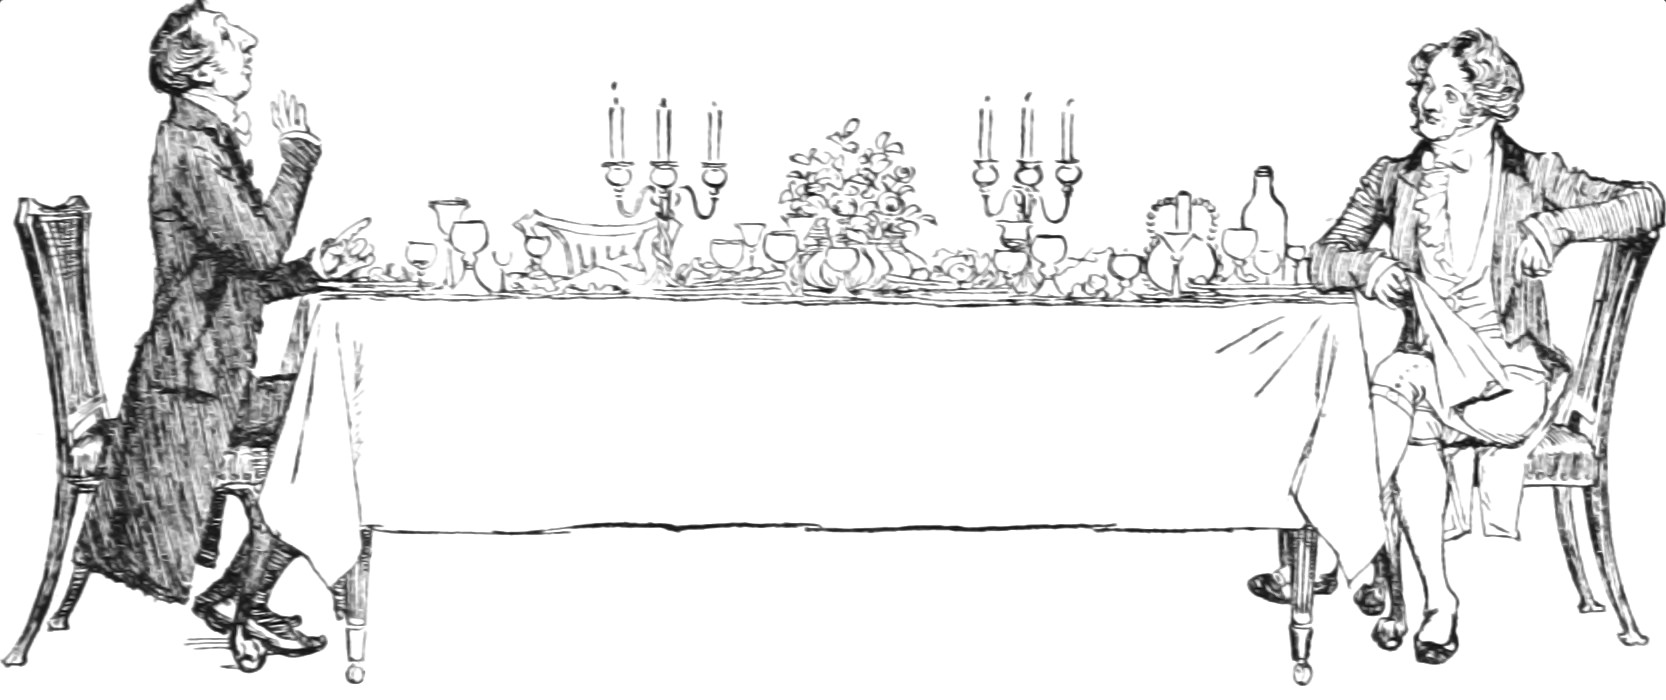
\includegraphics[width=\linewidth]{14top}
\captionlistentry{Headpiece to Chapter \thechapter}
\end{figure}

\lettrine[lines=5,image=true,lhang=.1]{initials/chap14d}{uring}  dinner, Mr Bennet scarcely spoke at all; but when the servants were withdrawn, he thought it time to have some conversation with his guest, and therefore started a subject in which he expected him to shine, by observing that he seemed very fortunate in his patroness. Lady Catherine de Bourgh's attention to his wishes, and consideration for his comfort, appeared very remarkable. Mr Bennet could not have chosen better. Mr Collins was eloquent in her praise. The subject elevated him to more than usual solemnity of manner; and with a most important aspect he protested that he had never in his life witnessed such behaviour in a person of rank—such affability and condescension, as he had himself experienced from Lady Catherine. She had been graciously pleased to approve of both the discourses which he had already had the honour of preaching before her. She had also asked him twice to dine at Rosings, and had sent for him only the Saturday before, to make up her pool of quadrille in the evening. Lady Catherine was reckoned proud by many people, he knew, but \textit{he} had never seen anything but affability in her. She had always spoken to him as she would to any other gentleman; she made not the smallest objection to his joining in the society of the neighbourhood, nor to his leaving his parish occasionally for a week or two to visit his relations. She had even condescended to advise him to marry as soon as he could, provided he chose with discretion; and had once paid him a visit in his humble parsonage, where she had perfectly approved all the alterations he had been making, and had even vouchsafed to suggest some herself,—some shelves in the closets upstairs.

<That is all very proper and civil, I am sure,> said Mrs Bennet, <and I dare say she is a very agreeable woman. It is a pity that great ladies in general are not more like her. Does she live near you, sir?>

<The garden in which stands my humble abode is separated only by a lane from Rosings Park, her Ladyship's residence.>

<I think you said she was a widow, sir? has she any family?>

<She has one only daughter, the heiress of Rosings, and of very extensive property.>

<Ah,> cried Mrs Bennet, shaking her head, <then she is better off than many girls. And what sort of young lady is she? Is she handsome?>

<She is a most charming young lady, indeed. Lady Catherine herself says that, in point of true beauty, Miss de Bourgh is far superior to the handsomest of her sex; because there is that in her features which marks the young woman of distinguished birth. She is unfortunately of a sickly constitution, which has prevented her making that progress in many accomplishments which she could not otherwise have failed of, as I am informed by the lady who superintended her education, and who still resides with them. But she is perfectly amiable, and often condescends to drive by my humble abode in her little phaeton and ponies.>

<Has she been presented? I do not remember her name among the ladies at court.>

<Her indifferent state of health unhappily prevents her being in town; and by that means, as I told Lady Catherine myself one day, has deprived the British Court of its brightest ornament. Her Ladyship seemed pleased with the idea; and you may imagine that I am happy on every occasion to offer those little delicate compliments which are always acceptable to ladies. I have more than once observed to Lady Catherine, that her charming daughter seemed born to be a duchess; and that the most elevated rank, instead of giving her consequence, would be adorned by her. These are the kind of little things which please her Ladyship, and it is a sort of attention which I conceive myself peculiarly bound to pay.>

<You judge very properly,> said Mr Bennet; <and it is happy for you that you possess the talent of flattering with delicacy. May I ask whether these pleasing attentions proceed from the impulse of the moment, or are the result of previous study?>

<They arise chiefly from what is passing at the time; and though I sometimes amuse myself with suggesting and arranging such little elegant compliments as may be adapted to ordinary occasions, I always wish to give them as unstudied an air as possible.>

Mr Bennet's expectations were fully answered. His cousin was as absurd as he had hoped; and he listened to him with the keenest enjoyment, maintaining at the same time the most resolute composure of countenance, and, except in an occasional glance at Elizabeth, requiring no partner in his pleasure.

\begin{figure}[tbh]
\centering
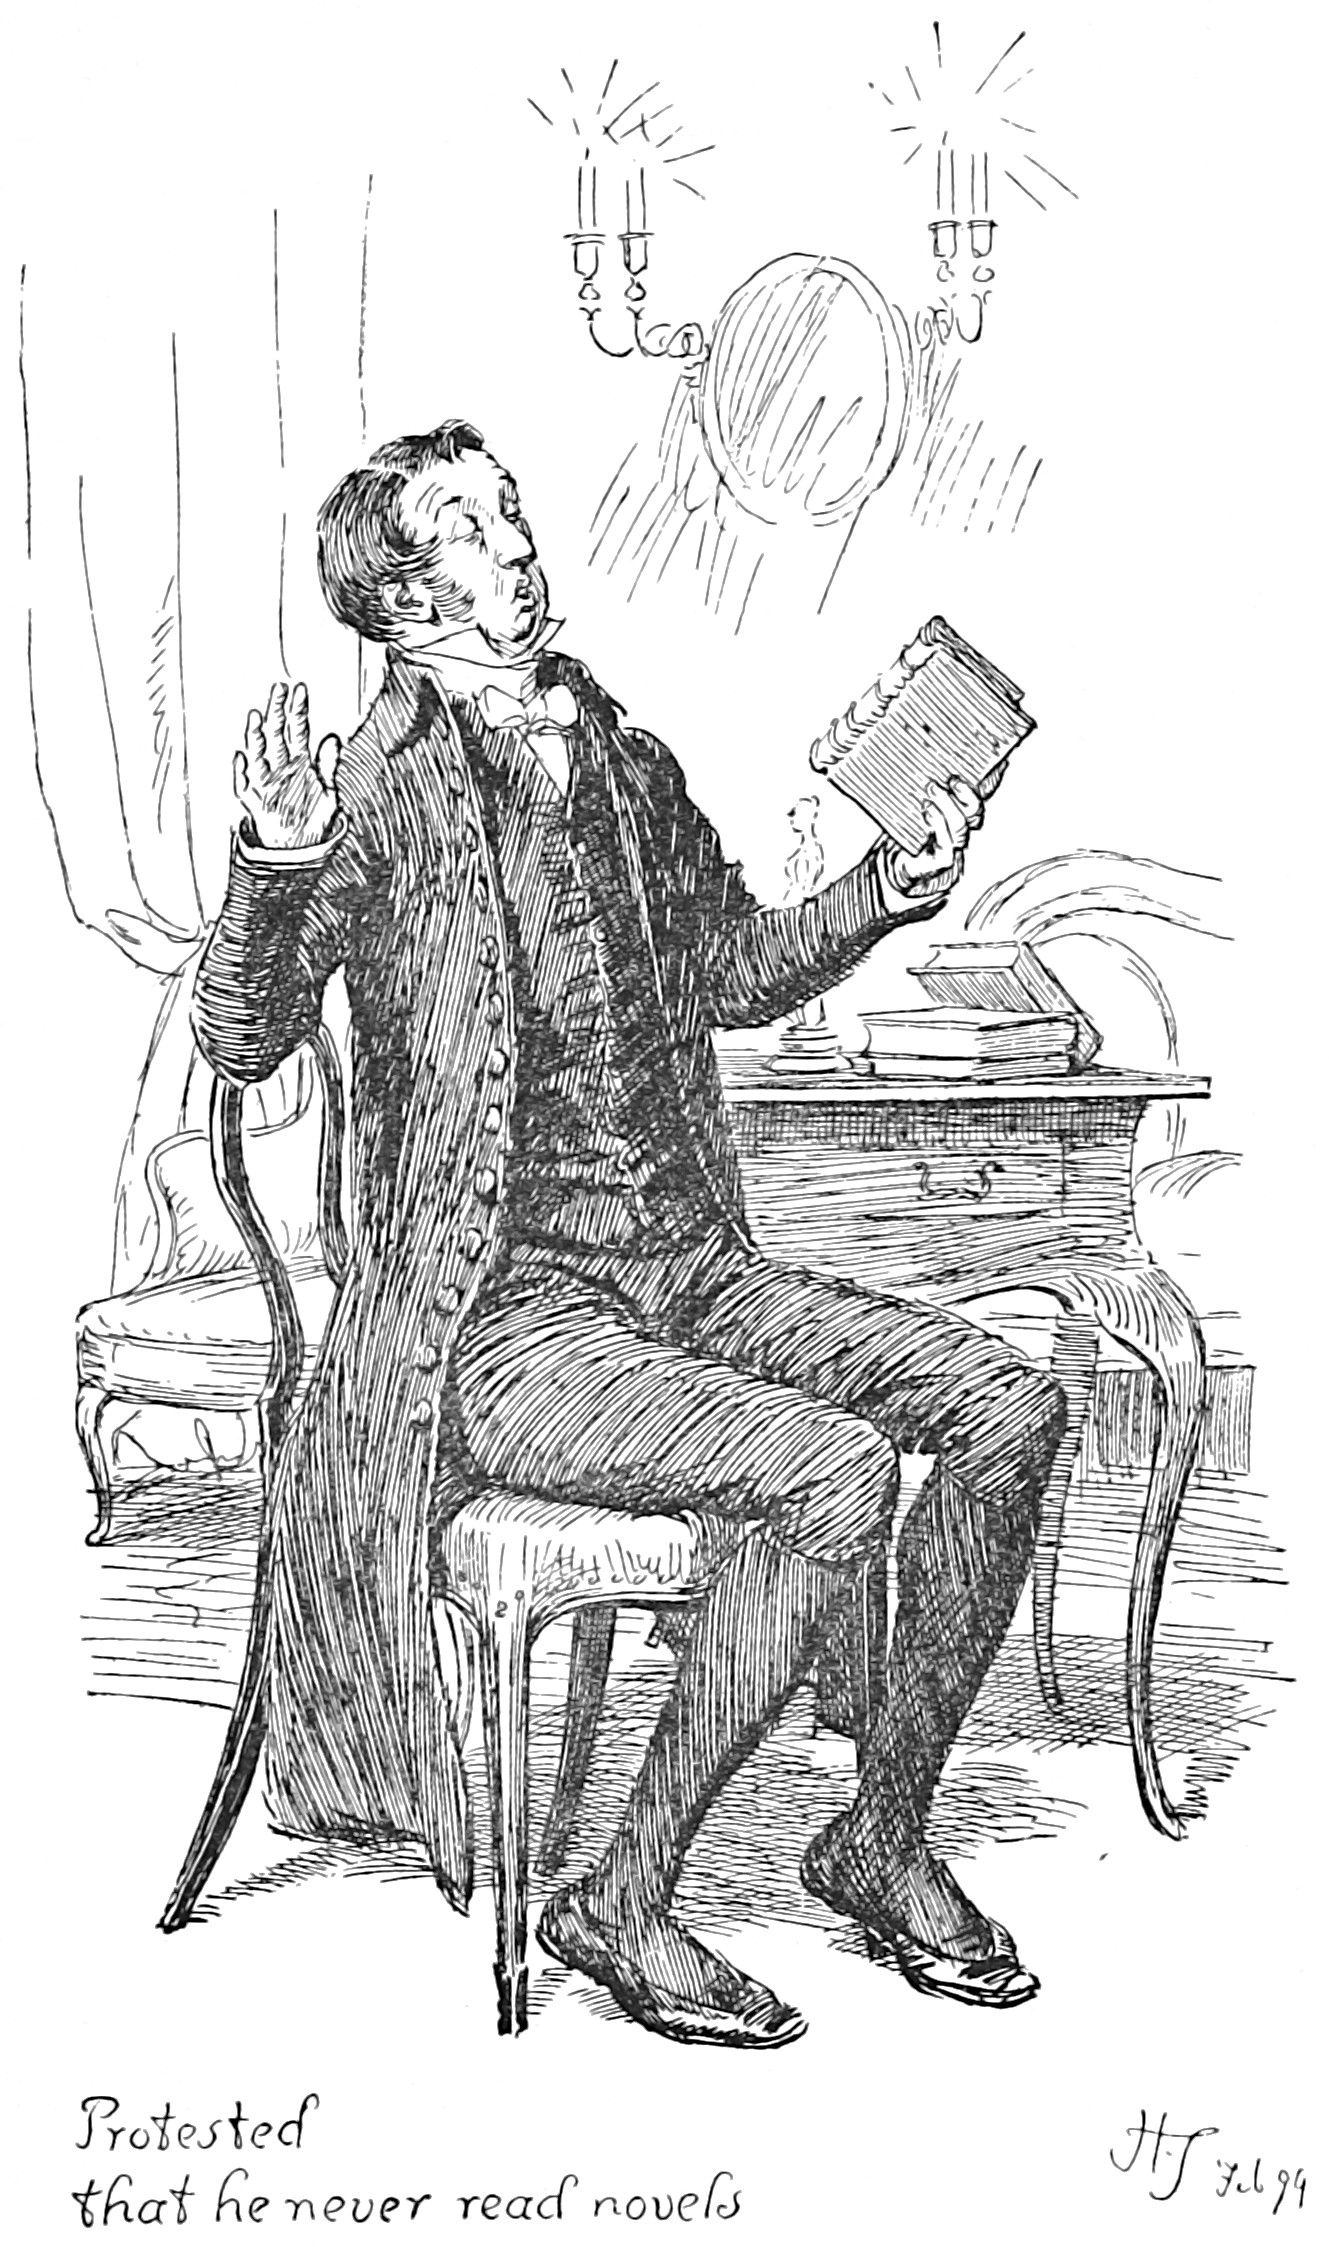
\includegraphics[width=.6\linewidth]{14novels}
\captionlistentry{Protested that he never read novels}
\end{figure}

By tea-time, however, the dose had been enough, and Mr Bennet was glad to take his guest into the drawing-room again, and when tea was over, glad to invite him to read aloud to the ladies. Mr Collins readily assented, and a book was produced; but on beholding it (for everything announced it to be from a circulating library) he started back, and, begging pardon, protested that he never read novels. Kitty stared at him, and Lydia exclaimed. Other books were produced, and after some deliberation he chose <Fordyce's Sermons.> Lydia gaped as he opened the volume; and before he had, with very monotonous solemnity, read three pages, she interrupted him with,—

<Do you know, mamma, that my uncle Philips talks of turning away Richard? and if he does, Colonel Forster will hire him. My aunt told me so herself on Saturday. I shall walk to Meryton to-morrow to hear more about it, and to ask when Mr Denny comes back from town.>

Lydia was bid by her two eldest sisters to hold her tongue; but Mr Collins, much offended, laid aside his book, and said,—

<I have often observed how little young ladies are interested by books of a serious stamp, though written solely for their benefit. It amazes me, I confess; for certainly there can be nothing so advantageous to them as instruction. But I will no longer importune my young cousin.>

Then, turning to Mr Bennet, he offered himself as his antagonist at backgammon. Mr Bennet accepted the challenge, observing that he acted very wisely in leaving the girls to their own trifling amusements. Mrs Bennet and her daughters apologized most civilly for Lydia's interruption, and promised that it should not occur again, if he would resume his book; but Mr Collins, after assuring them that he bore his young cousin no ill-will, and should never resent her behaviour as any affront, seated himself at another table with Mr Bennet, and prepared for backgammon.